% ****************************************************************************************************
% Chapter 3: Real Data, MIMIC-IV-ED
% ****************************************************************************************************

\chapter{Real Data: MIMIC-IV-ED}
\label{ch:mimic}

The decision to pivot to real clinical data was made in the second week of the project, and it was not immediate. This chapter describes how the pivot actually happened, the slow accumulation of suspicion, the practical steps of obtaining credentialed access, and the first careful exploration of the new dataset. It is partly a technical description and partly a narrative, because the choices made at this stage shaped everything that followed.

\section{Why Not Act Immediately}

When I first noticed that adding text features jumped the model from F1 = 0.87 to F1 = 0.998, the correct scientific response would have been to stop and investigate. I did not do that immediately. I spent several days continuing to improve the pipeline on the Kaggle data, adding more features, tuning hyperparameters, trying different embedding models. The scores kept rising toward the ceiling. In retrospect, this was wasted effort, but at the time it was easy to rationalise: perhaps the dataset was real and the text was simply very informative. Perhaps nurses really did write chief complaints with such clear severity markers. Perhaps I was being paranoid.

The moment of commitment came roughly one week into the project. I had independently reproduced the keyword analysis shown in Chapter~\ref{ch:discovery}, the 99.8\% verbatim match between train and test complaints, and the non-significant chi-squared test on the body-system column. I had also checked the Kaggle discussion forum and noticed that other competitors were reporting similar findings. At that point the leakage was no longer a suspicion but a documented property of the dataset.

I also briefly entertained a more charitable interpretation. The Laitinen-Fredriksson Foundation competition is judged on a rubric that explicitly rewards novelty and insight, not leaderboard position. One reading of the synthetic leakage is that it was deliberate, a test of whether competitors would notice the flaw and engage with it, or simply take the easy 0.999 and stop. I cannot know whether this was the organisers' intent, but it shaped my strategy. If the competition rewarded rigorous clinical ML over leaderboard gaming, then the correct response was to build the real thing.

\begin{remarkbox}[On Deciding Alone]
This was a solo decision, but not made in isolation. Throughout the project I benefited from conversations with a friend, a theoretical physicist now working in machine learning, who provided the kind of external perspective that research physicists recognise from years of journal club. Having someone outside the immediate work who asks good questions, pushes back on fuzzy thinking, and shares the enthusiasm for doing things properly is, in my experience, more valuable than most formal research supervision. I record this here because methodological descriptions often omit the informal scaffolding that actually keeps projects honest.
\end{remarkbox}

\section{Why MIMIC-IV-ED}

Several real clinical datasets could in principle have been used. I focused exclusively on MIMIC-IV-ED, and this focus deserves explanation.

The Medical Information Mart for Intensive Care (MIMIC) is a family of de-identified electronic health record datasets from the Beth Israel Deaconess Medical Center (BIDMC) in Boston. The original MIMIC-III dataset, released in 2016, contained roughly 40,000 ICU patients and became the most widely used clinical ML benchmark in the world. MIMIC-IV, released in stages from 2020 onward, extends the dataset with more patients, more modules, and a more carefully documented data model \citep{johnson2023mimiciv}. MIMIC-IV-ED is the emergency department module: 448,972 ED visits with triage information, vital signs, medication reconciliation, diagnoses, and discharge disposition \citep{xie2022mimicived}. I used version 3.1, the most recent at the time of this project.

Three specific properties made MIMIC-IV-ED the right choice for my work.

First, it contains 5-level ESI acuity labels for every visit. This is the actual target I wanted to predict, not a proxy like admission or mortality. As I noted in Chapter~\ref{ch:triage-problem}, most published ML triage systems predict binary outcomes rather than the full ESI scale, so data with real ESI labels at this volume is unusual.

Second, the credentialing process is standardised, transparent, and accessible to independent researchers. Other real ED datasets exist, the US National Hospital Ambulatory Medical Care Survey (NHAMCS) has limited features, the eICU Collaborative Research Database covers ICUs rather than EDs, and large national registries like the Korean NEDIS are not publicly accessible. MIMIC-IV-ED is one of the few datasets where an individual outside a hospital affiliation can, with reasonable effort, obtain legitimate access to real patient data.

Third, the institutional link to clinical NLP tooling is unusually clean. The Bio\_ClinicalBERT language model \citep{alsentzer2019clinicalbert}, which I discuss at length in Chapter~\ref{ch:embeddings}, was pretrained on clinical notes from the same BIDMC system that generated MIMIC-IV-ED. When I fine-tune ClinicalBERT on chief complaints from MIMIC-IV-ED, I am fine-tuning a model on text from the institution it was pretrained on. This minimises domain shift in ways that are harder to achieve with other combinations.

\begin{notebox}[Other Datasets I Did Not Use]
A thorough project would have validated methodology on multiple external datasets rather than a single institution. I did not do this, for a simple reason: obtaining MIMIC access and understanding the schema well enough to use it correctly took several weeks on its own. Adding a second credentialed dataset, with its own CITI requirements, data use agreements, and schema idiosyncrasies, would have consumed time I did not have. I flag this as a limitation in Chapter~\ref{ch:limitations} and note that external validation on, for example, eICU or NHAMCS would be a natural extension of this work.
\end{notebox}

\section{The Credentialing Process}

Obtaining MIMIC-IV-ED is not immediate. It requires registering a PhysioNet account, completing the Collaborative Institutional Training Initiative (CITI) course on human-subjects research (specifically the \emph{Data or Specimens Only Research} curriculum, covering the Belmont Report, HIPAA, de-identification standards, and the history of ethical violations in medical research), submitting a credentialing application with a short description of intended research and a reference who can vouch for the applicant's research seriousness, and signing the MIMIC-IV-ED Data Use Agreement. The CITI course takes about four hours and the certificate is valid for three years. PhysioNet review can take a few days during quiet periods and longer when busy. From starting the CITI course to having the data downloaded, the elapsed time in my case was about a week, and a realistic plan is to allow roughly two weeks between deciding to use MIMIC and having clean intermediate results. I mention this explicitly because the documentation tends to make the process sound faster than it is in practice, and because the gates themselves are the point: they exist to ensure that researchers using patient data understand their responsibilities. I recommend taking the course seriously rather than clicking through; several of its modules reshape how one thinks about downstream obligations in ways that become relevant in Chapter~\ref{ch:fairness}.

\section{First Contact with the Data}

Once the dataset was downloaded, the next question was what was actually in it. MIMIC-IV-ED consists of several tables linked by patient and visit identifiers, and MIMIC-IV (the parent dataset) contains many more. A first glance at the file listing is disorienting: dozens of CSV files, some hundreds of megabytes in size, with cryptic names like \texttt{edstays.csv}, \texttt{triage.csv}, \texttt{medrecon.csv}, \texttt{pyxis.csv}, \texttt{diagnoses\_icd.csv}. The temptation is to start loading and modelling immediately. I resisted this, and it was one of the better decisions of the project.

\subsection*{Why Start with Exploration}

Coming from a background outside healthcare, many of the features required interpretation before they could be used. What is a \texttt{stay\_id} and how does it relate to a \texttt{hadm\_id}? What does it mean for \texttt{arrival\_transport} to be coded as \texttt{AMBULANCE} versus \texttt{WALK IN} versus \texttt{UNKNOWN}? Why does \texttt{temperature} sometimes have values like 97.6 and sometimes 36.4? (The answer: Fahrenheit versus Celsius, with no unit column, the researcher has to detect and harmonise.) Why is \texttt{pain} sometimes \texttt{-1}? (Because the triage form allows ``unable to assess'' to be coded as a numeric flag, which must be recoded to missing before any analysis.)

These are not obscure details. Every one of them, if mishandled, silently corrupts downstream analysis. A model trained on mixed Fahrenheit and Celsius temperatures will learn an artefact of data entry conventions rather than patient physiology. A pain score where \texttt{-1} is treated as a valid numeric value will pull every analysis downward. The only reliable way to catch these issues is to look at the data carefully before modelling.

\begin{highlightbox}
\textbf{Methodological note.} Before applying any statistical or machine learning technique to a new dataset, I strongly recommend building a simple exploratory dashboard that allows interactive inspection of distributions, missingness patterns, correlations, and individual records. The time spent is repaid many times over in avoided errors downstream. For someone without a clinical background, this exploration phase is also an education: the dataset teaches you what the features mean, how they are used in practice, and which of your assumptions need revision.
\end{highlightbox}

\subsection*{The Exploration Dashboard}

I spent approximately three days building a Dash-based dashboard for MIMIC-IV-ED exploration, separate from any modelling code. The dashboard allowed filtering by ESI level, age group, arrival mode, and acuity, and displayed distributions of every feature in the filtered subset. Individual patients could be clicked to see their complete record. Correlations between features and the target could be visualised interactively.

The results of this exploration were revealing. Missing vital signs were not random, they correlated strongly with acuity level, with critically ill patients more likely to have missing values because their condition made measurement difficult or skipped. Temperature was missing in a large fraction of ESI-1 cases, where the priority is immediate stabilisation rather than temperature measurement. Pain scores were missing in unconscious patients almost by definition. These missingness patterns are themselves signal, and I incorporated them as explicit missingness-flag features in the final model (see Chapter~\ref{ch:features}).

The chief complaint text, in the exploration dashboard, looked completely different from the Kaggle synthetic version. There were no systematic severity adjectives. Complaints like ``63M c/o chest pain onset 2h'' or ``altered MS, found down by family, unclear duration'' were common. The vocabulary was idiosyncratic, with abbreviations that varied between nurses and shifts. This was unmistakably real clinical text.

\section{The Cohort}

MIMIC-IV-ED v3.1 contains 425,087 ED visits linked to 216,877 unique patients. After excluding visits with missing ESI labels (roughly 1.6\%), the analytic cohort consists of 418,100 ED visits. This is the cohort used throughout the remainder of this report.

I did not restrict by age. MIMIC-IV-ED includes both adult and pediatric patients, and I kept all of them. In MIMIC, patients under 18 are recorded with their true age, while adult ages at admission are anchored to a reference year and shifted in blocks to de-identify birth dates. The \texttt{anchor\_age} field gives age at the anchor year, and ages at later visits must be computed from the anchor offset. This de-identification scheme preserves longitudinal structure within a patient but makes some naive age computations subtly wrong. I used the \texttt{anchor\_age} at the visit year throughout.

Multiple visits per patient are common. The median patient has one ED visit in the dataset, but some patients have dozens. This raised a design question: should features that aggregate over prior visits (number of prior ED visits, prior diagnoses, prior severity codes) be computed per visit, with careful attention to temporal ordering to avoid leakage?

I chose the leakage-safe path. All history features are computed using group-wise \texttt{cumcount} and \texttt{cummax + shift(1)} operations, which ensure that each visit's feature values depend only on strictly prior visits for the same patient. If a patient's third ED visit happens on 15 June 2180, the features describing their history at that visit include data from their first and second visits but nothing from the third visit itself or any later visit. This is the correct behaviour for a prediction system: at the moment of triage, the system has access only to information that existed before that moment.

\begin{notebox}[What Is Temporal Leakage?]
Temporal leakage occurs when features computed for a given visit accidentally include information from that visit or from later visits. A naive implementation of ``number of prior ED visits'' might count all visits for this patient in the dataset, including the current one and future ones. At prediction time this number would be unavailable. A model trained on leaky history features will score well in cross-validation and fail in deployment.

The \texttt{cumcount} operation, computed within each patient group sorted by visit date, avoids this by counting only strictly prior visits. The \texttt{cummax + shift(1)} pattern does the same for maximum-over-history features. These patterns are straightforward to implement correctly, but they are easy to get wrong, and the consequences are silent, the model does not crash, it just overfits.
\end{notebox}

\section{The Class Distribution Shift}

The first substantive difference between MIMIC-IV-ED and the Kaggle synthetic data became clear immediately: the class distributions are radically different. Figure~\ref{fig:class-distribution-comparison} repeats the comparison from Chapter~\ref{ch:discovery}, now with the interpretation made explicit.

In the Kaggle data, the ESI distribution is roughly bell-shaped: ESI-3 dominates at 36\%, flanked by ESI-4 at 29\% and ESI-2 at 17\%, with the extremes at 4\% (ESI-1) and 14\% (ESI-5). This is not implausible as a summary of an idealised ED population.

In the real MIMIC-IV-ED data, ESI-3 dominates even more strongly at 54\%, ESI-2 is at 33\%, and the tails collapse: ESI-1 is rare at 6\%, ESI-4 at 7\%, and ESI-5 is nearly absent at 0.3\%. The ESI-5 category is so sparse that it contains only about 1,100 patients across the entire 418,100-visit cohort.

This is clinically plausible: BIDMC is a large urban academic medical centre with a trauma designation. Patients who would be ESI-5 (truly non-urgent, no resources needed) typically do not come to this kind of ED. They go to urgent care, primary care, or ambulatory clinics. The MIMIC-IV-ED distribution reflects the case mix of a tertiary academic hospital, not of an average ED across all settings.

The implication for modelling is substantial. Any approach that works well on the Kaggle distribution may perform differently on MIMIC, particularly for the ESI-5 class where a tiny sample size caps what any classifier can achieve. This became an important caveat throughout the project. My best MIMIC F1 for ESI-5 is 0.260, which sounds poor in isolation but is constrained by the 0.3\% prevalence, with roughly 1,100 positives across five folds, the sampling noise alone is substantial.

\begin{figure}[htbp]
 \centering
 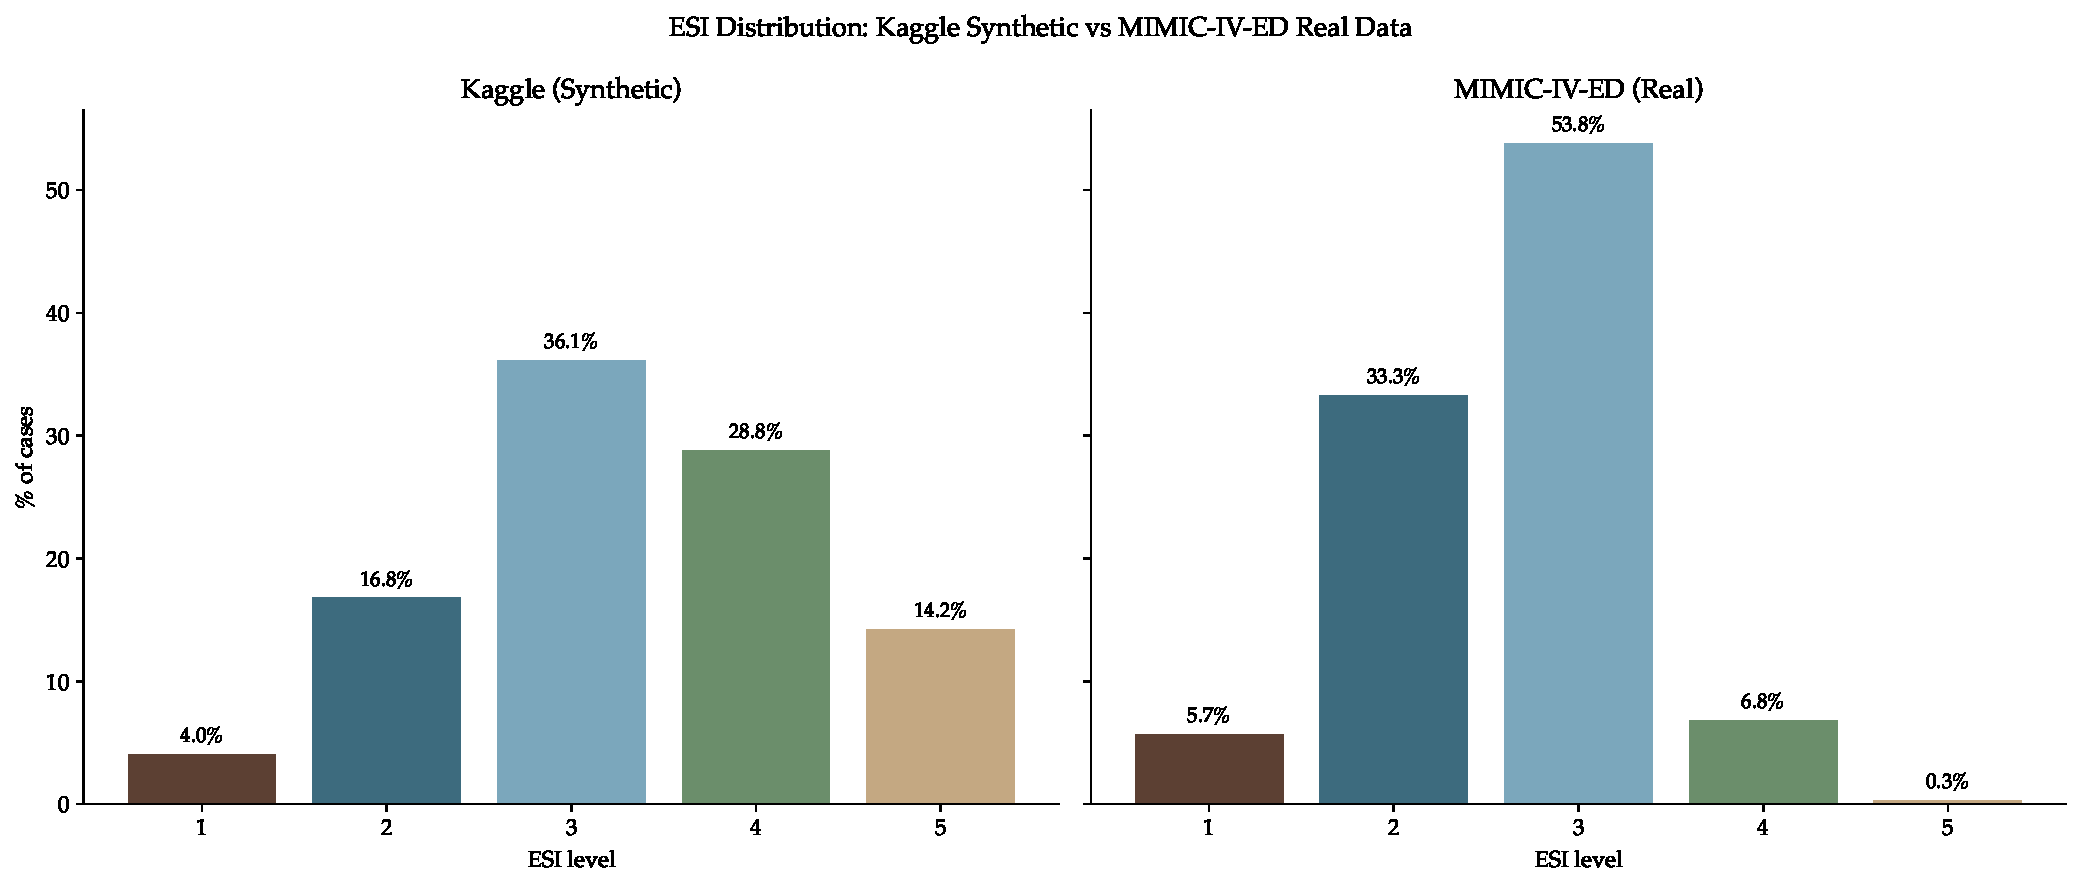
\includegraphics[width=0.9\textwidth]{figures/class_distribution_comparison.pdf}
 \caption[ESI distribution: synthetic vs real]{ESI acuity level distributions for the Kaggle synthetic competition data (left) and MIMIC-IV-ED (right). The synthetic data is roughly bell-shaped around ESI-3. The real clinical data is strongly skewed: ESI-3 and ESI-2 together account for 87\% of visits, while ESI-5 patients are nearly absent (0.3\%). The difference reflects the case mix of a tertiary academic medical centre, and has substantial implications for model evaluation.}
 \label{fig:class-distribution-comparison}
\end{figure}

\section{The Data Model}

MIMIC-IV-ED is distributed as a relational database, typically provided as CSV files that correspond to tables. Understanding the relationships between tables is essential before any feature engineering. I spent some time drawing the schema by hand before writing any join code. The main ED tables (\texttt{edstays}, \texttt{triage}, \texttt{medrecon}, \texttt{diagnosis}, \texttt{pyxis}) join via \texttt{stay\_id}, link to patient-level history via \texttt{subject\_id}, and link to parent MIMIC-IV hospital admissions (\texttt{patients}, \texttt{admissions}, \texttt{diagnoses\_icd}, \texttt{drgcodes}) via \texttt{hadm\_id}. \texttt{pyxis} (medication dispensing during the stay) is post-triage and therefore excluded to prevent leakage.

The key tables I used are:

\begin{itemize}
 \item \texttt{edstays}, one row per ED visit, with admission and discharge timestamps, arrival mode, and disposition.
 \item \texttt{triage}, one row per ED visit, with vital signs measured at triage, chief complaint text, and the ESI acuity label. This is the primary table for the prediction task.
 \item \texttt{medrecon}, medication reconciliation, one row per pre-admission medication per visit. Used to construct therapeutic-class flags.
 \item \texttt{diagnosis}, one row per ICD diagnosis code per visit. Used for the Charlson comorbidity composite, computed from strictly prior visits only.
 \item \texttt{patients} (from MIMIC-IV), one row per patient, with demographic information and \texttt{anchor\_age}.
 \item \texttt{admissions} (from MIMIC-IV), one row per hospital admission, used to link ED visits to subsequent hospital stays and to compute prior-admission history features.
 \item \texttt{diagnoses\_icd} (from MIMIC-IV), historical diagnoses across all encounters, used for Charlson comorbidity flags.
\end{itemize}

I explicitly did not use \texttt{pyxis} (medication dispensing records from during the hospital stay), \texttt{disposition} (how the ED visit concluded), or any other post-triage feature. Including these would have produced better accuracy numbers but would have been leakage: at the time of triage, none of this information is available. The entire feature engineering pipeline, described in Chapter~\ref{ch:features}, is built on this principle.

\section{What Comes Next}

Having the data, understanding the schema, and settling the cohort was, in retrospect, half the work. The other half, feature engineering, modelling, evaluation, safety analysis, fairness audits, explainability, is the subject of the remaining chapters. But all of it is downstream of the decisions made in this chapter. The cohort is 418,100 visits. The target is the 5-level ESI label. The class distribution is dominated by ESI-3 with a nearly-empty ESI-5 category. All history features are leakage-safe. All post-triage features are excluded. These ground rules are carried forward without further discussion.

I turn now to the features themselves: the 65 variables that, together with the chief complaint text, form the input to the model.
